% Source: graduate-coursework/Research/Intro_to_Agents/handouts/Part3_Basic_Usage.tex

\documentclass[border=4pt]{standalone}
\usepackage[T1]{fontenc}
\usepackage{graphicx}
\usepackage{lmodern}
\usepackage{tikz}
\usepackage{xcolor}
\usetikzlibrary{shapes.geometric,arrows.meta,positioning,calc,fit,backgrounds,decorations.pathreplacing}

\definecolor{UofSCGarnet}{HTML}{73000a}
\definecolor{UofSCBlack}{HTML}{000000}
\definecolor{UofSCWhite}{HTML}{ffffff}
\definecolor{UofSCRose}{HTML}{CC2E40}
\definecolor{UofSCAtlantic}{HTML}{466A9F}
\definecolor{UofSCCongaree}{HTML}{1F414D}
\definecolor{UofSCHorseshoe}{HTML}{65780B}
\definecolor{UofSCGrass}{HTML}{CED318}
\definecolor{UofSCHoneycomb}{HTML}{A49137}
\definecolor{UofSC90Black}{HTML}{363636}
\definecolor{UofSC70Black}{HTML}{5C5C5C}
\definecolor{UofSC50Black}{HTML}{A2A2A2}
\definecolor{UofSCWarmGrey}{HTML}{676156}
\definecolor{UofSCSandstorm}{HTML}{FFF2E3}
\definecolor{UofSCDarkGarnet}{HTML}{570008}
\definecolor{UofSCAzalea}{HTML}{844247}

\tikzset{
    % Sharp-cornered boxes
    process/.style={
        rectangle,
        draw=UofSCBlack,
        thick,
        fill=UofSCWhite,
        text=UofSCBlack,
        minimum width=3cm,
        minimum height=0.8cm,
        align=center,
        font=\small
    },
    process highlight/.style={
        process,
        fill=UofSCGarnet,
        text=UofSCWhite
    },
    process secondary/.style={
        process,
        fill=UofSCAtlantic,
        text=UofSCWhite
    },
    process tertiary/.style={
        process,
        fill=UofSCCongaree,
        text=UofSCWhite
    },
    arrow/.style={
        ->,
        >=Stealth,
        thick,
        color=UofSCBlack
    },
    arrow garnet/.style={
        arrow,
        color=UofSCGarnet
    },
    label box/.style={
        rectangle,
        draw=none,
        fill=UofSCSandstorm,
        text=UofSCBlack,
        font=\scriptsize,
        align=center
    },
    decision/.style={
        diamond,
        draw=UofSCBlack,
        thick,
        fill=UofSCHoneycomb,
        text=UofSCBlack,
        minimum width=2cm,
        minimum height=1cm,
        align=center,
        font=\small,
        aspect=2
    }
}

\begin{document}
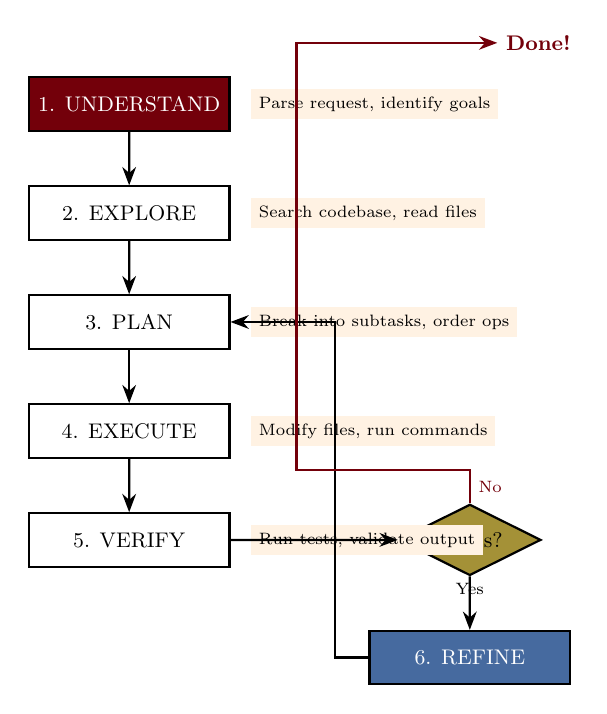
\begin{tikzpicture}[node distance=0.8cm and 0.5cm, scale=0.85, transform shape]
        % Nodes
        \node[process highlight] (understand) {1. UNDERSTAND};
        \node[process, below=of understand] (explore) {2. EXPLORE};
        \node[process, below=of explore] (plan) {3. PLAN};
        \node[process, below=of plan] (execute) {4. EXECUTE};
        \node[process, below=of execute] (verify) {5. VERIFY};
        \node[decision, right=2.5cm of verify] (issues) {Issues?};
        \node[process secondary, below=of issues] (refine) {6. REFINE};

        % Descriptions
        \node[label box, right=0.3cm of understand] {Parse request, identify goals};
        \node[label box, right=0.3cm of explore] {Search codebase, read files};
        \node[label box, right=0.3cm of plan] {Break into subtasks, order ops};
        \node[label box, right=0.3cm of execute] {Modify files, run commands};
        \node[label box, right=0.3cm of verify] {Run tests, validate output};

        % Arrows
        \draw[arrow] (understand) -- (explore);
        \draw[arrow] (explore) -- (plan);
        \draw[arrow] (plan) -- (execute);
        \draw[arrow] (execute) -- (verify);
        \draw[arrow] (verify) -- (issues);
        \draw[arrow] (issues) -- node[above, font=\scriptsize] {Yes} (refine);
        \draw[arrow] (refine.west) -- ++(-0.5,0) |- (plan.east);
        \draw[arrow garnet] (issues.north) |- node[right, font=\scriptsize, pos=0.25] {No} ++(0,0.5) -| ($(understand.north)+(2.5,0.5)$) -- ++(3,0) node[right, font=\small\bfseries, text=UofSCGarnet] {Done!};
    \end{tikzpicture}
\end{document}
